%%novalidate
\newpage
\section{Destination Tickets \& Effective Resistance}

\subsection{Destination Tickets \& Winning}
An obvious strategy in \textit{Ticket to Ride} is to collect
Destination Tickets and buy routes so as to connect them.
We investigate the effect of collecting Destination Tickets
on winning the game.
We simulate 10,000 two-player and 10,000 four-player games
using Silva et al.'s program.
For each Destination Ticket, we calculate the proportion of 
games that the player holding the Destination Ticket won.
For example, players in two-player games with Phoenix to Portland
won almost exactly half of their games.
Our results appear in \cref{fig:tickets}.

\end{multicols}
\begin{figure}[h]
\centering
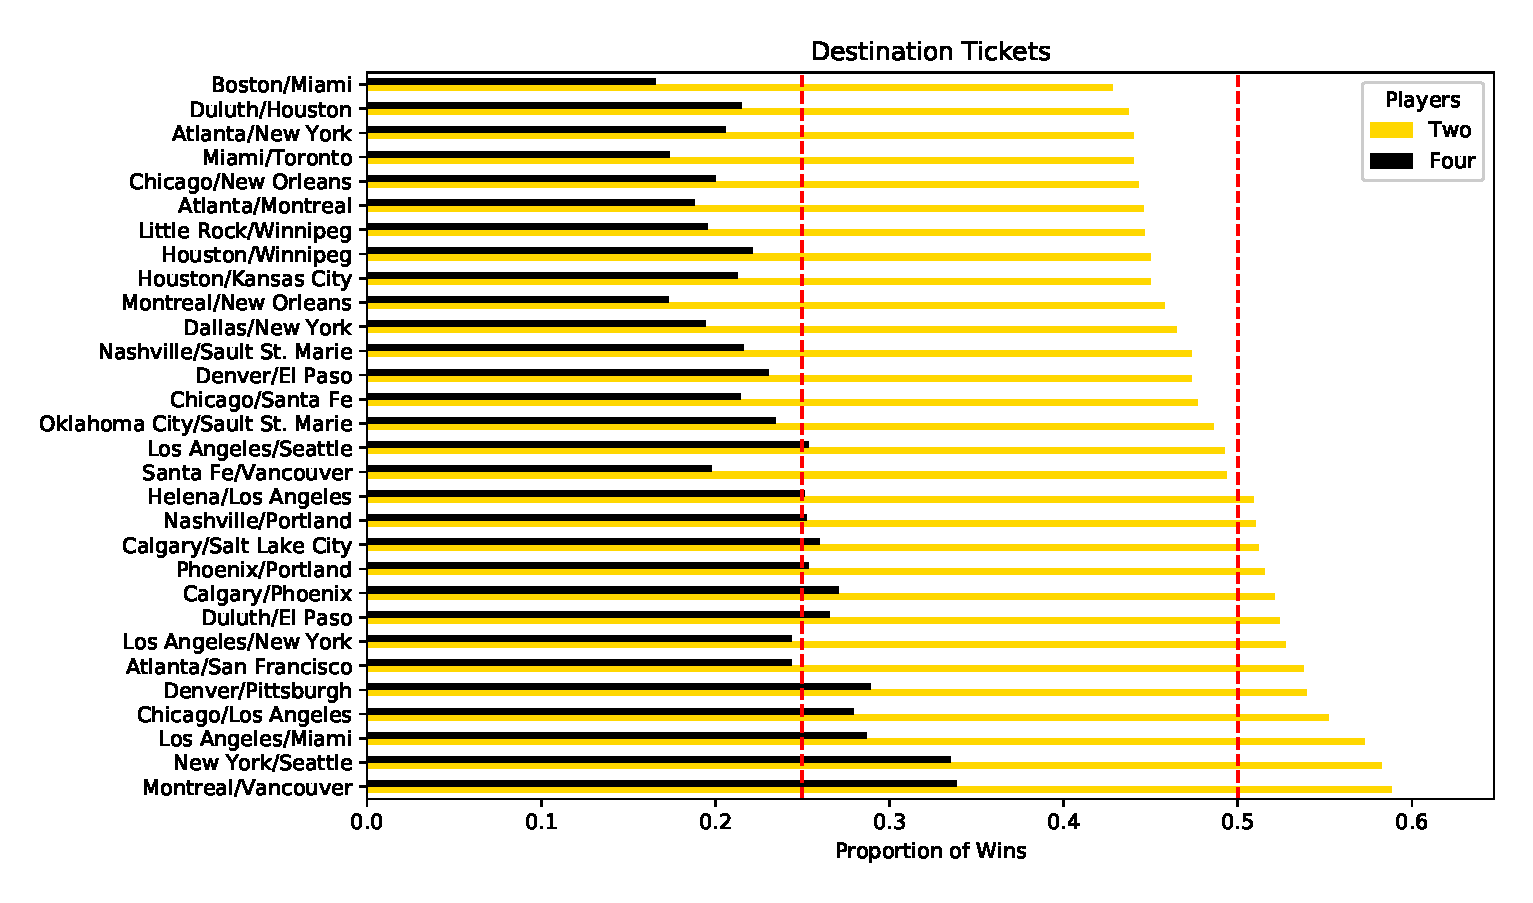
\includegraphics[scale=.8]{figures/destination_tickets}
\caption{For each Destination Ticket,
the proportion of two-player and four-player games that 
the player with the Destination Ticket won.
The vertical red lines at $1/4$ and $1/2$ represent
the expected proportion of games players would win
if Destination Tickets had no effect.}
\label{fig:tickets}
\end{figure}
\begin{multicols}{2}

The vertical red lines at $1/4$ and $1/2$ indicate
the expected proportion of wins if Destination Tickets
had no effect on winning: players in two-player games
would win half the time and players in four-player games
would win a quarter of the time.

Remarkably, there are no Destination Tickets in four-player
games that win more than $25\%$ of all games.
This would be impossible if all players had the same number
of Destination Tickets because \textit{some} player must win every
game.
Therefore the implication is that players who spend their
turns collecting more Destination Tickets win less frequently
than those who take Train Cards or claim routes.
Within the set of Destination Tickets in four-player games,
some still do even worse.
New York to Seattle, Los Angeles to New York, Los Angeles to Miami,
and Montreal to Vancouver have especially low win rates.
A quick inspection of \cref{fig:board} shows that all four pairs of cities
are particularly far apart (in terms of both geography and the
length of the shortest paths between them).
Perhaps these longer Destination Tickets are harder to connect and,
in the common case that players cannot connect them, subtract an insurmountable
number of points from players' final scores.

Destination Tickets in two-player games also mostly fall
below the threshold of wins we would expect if there were
no relationship between winning and Destination Tickets.
But, unlike four-player games, some Destination Tickets
win more than expected: Montreal to Vancouver,
Los Angeles to Miami, Chicago to Los Angeles, and
Denver to Pittsburgh.
Ironically, the cities that won the least often in four-player
games now win the most often in two-player games.
Perhaps the longer Destination Tickets are easier
to connect in two-player than four-player games
and, unlike the other Destination Tickets, add
a substantial number of points to the final score.

We dive into the math to explore the deeper structure
of Destination Tickets.

\subsection{Effective Resistance}
The \textit{Ticket to Ride} board can conveniently
be thought of as a graph where cities represent
nodes and routes represent edges.
Therefore to analyze the difficulty of connecting a
pair of cities we can frame the problem in graph theoretic language.
One of the most powerful and natural measures
between two nodes on a graph is effective resistance
\cite{ellens2011effective}.
Imagine that the \textit{Ticket to Ride} board was
a large electrical circuit with a unit current
entering at city $a$ and leaving at city $b$.
Effective resistance is a measure
of how much work a current needs to exert
to get from $a$ to $b$.
In general, the number of paths and length of routes 
determine the effective resistance:
two cities with fewer paths and longer routes
have a higher effective resistance between them
than two cities with many paths and shorter routes.
We calculate the effective resistance for each 
Destination Ticket in order to gain insight
into what makes players with some Destination Tickets
win more often than players with other Destination Tickets.

On a small graph, effective resistance can be calculated
by repeatedly applying the following rules.
Consider two edges with resistances $r_1$ and $r_0$.
If the two edges are in series (edge 1 connects node $i$ to $j$
and edge 2 connects node $j$ to $k$), then the resistance between
$i$ and $i$ is $r_1 + r_2$.
If the two edges are in parallel (both edge 1 and edge 2 connect
node $i$ to $j$), then the resistance between $i$ and $j$
is $(1/r_1 + 1/r_2)^{-1}$.

On a large graph like the \textit{Ticket to Ride} board, 
the process becomes inefficient.
We instead use two separate algorithms to find the effective resistance
of Destination Tickets
\cite{ellens2011effective, wu2004theory}.
Both algorithms calculate the effective resistance by finding 
the eigenvalues of the Laplacian matrix for a given graph.
The Laplacian is the degree matrix $D$ minus the adjacency
matrix $A$ where $D_{i,i}$ is the weighted degree of node $i$
and $A_{i,j}$ is the resistance of the edges between nodes
$i$ and $j$.

We let the weight between two cities be the number
of trains of the route connecting them.
In the case that there are two routes between cities,
we let the weight be $(1/r + 1/r)^{-1}=r/2$ where
$r$ is the number of trains of each route.
Our results appear in \cref{fig:resistance4}
and \cref{fig:resistance4}.

\end{multicols}
\begin{figure}
    \centering
    \begin{subfigure}[b]{\textwidth}
        \includegraphics[scale=.65]{figures/resistance_four}
        \caption{Destination Tickets by their effective
        resistance and minimum path length and colored
        by the proportion of wins in four-player games.
        The line of best fit gives an approximation of the
        Destination Tickets that are better deals (above the line).
        Note: the $16^{th}$ Destination Ticket Portland/Phoenix is obscured
        by the $18^{th}$.}
        \label{fig:resistance4}
    \end{subfigure}
    \vfill
    \begin{subfigure}[b]{\textwidth}
        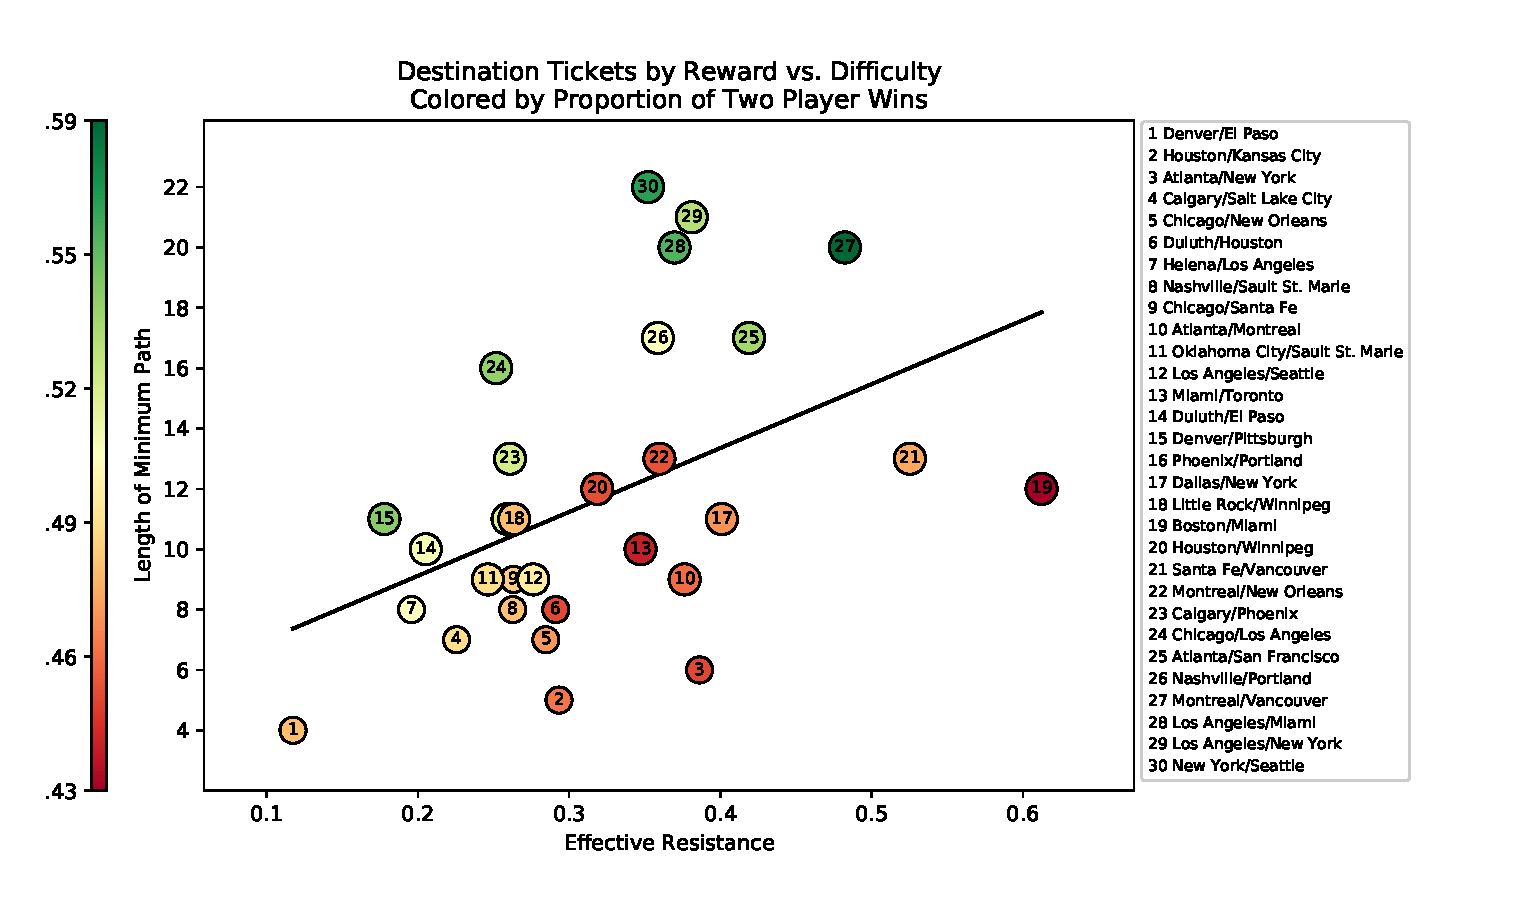
\includegraphics[scale=.65]{figures/resistance_two}
        \caption{\cref{fig:resistance4} colored by proportion
        of wins in two-player rather than four-player games.}
        \label{fig:resistance2}
    \end{subfigure}
\end{figure}
\begin{multicols}{2}

\end{multicols}
\begin{table}[]
\begin{tabular}{|c|l|l|l|l|}
\hline
\textbf{}                 & \textbf{Path Length} & \textbf{Two-player Wins} & \textbf{Four-player Wins} & \textbf{Best Fit Distance} \\ \hline
\textbf{Resistance}       & \textit{4.923e-02}   & \textit{3.667e-01}       & 7.798e-03                 & \textit{1.000e+00}         \\ \hline
\textbf{Path Length}      &                      & 1.491e-05                & 8.127e-18                 & 7.108e-14                  \\ \hline
\textbf{Two-player Wins}  &                      &                          & 1.108e-03                 & 2.878e-08                  \\ \hline
\textbf{Four-player Wins} &                      &                          &                           & 2.730e-09                  \\ \hline
\end{tabular}
\end{table}
\begin{multicols}{2}